\chapter{Design}



%You should concentrate on the more important aspects of the design. It is essential that an overview is presented before going into detail. As well as describing the design adopted it must also explain what other designs were considered and why they were rejected.

%The design should describe what you expected to do, and might also explain areas that you had to revise after some investigation.

%Typically, for an object-oriented design, the discussion will focus on the choice of objects and classes and the allocation of methods to classes. The use made of reusable components should be described and their source referenced. Particularly important decisions concerning data structures usually affect the architecture of a system and so should be described here.

%How much material you include on detailed design and implementation will depend very much on the nature of the project. It should not be padded out. Think about the significant aspects of your system. For example, describe the design of the user interface if it is a critical aspect of your system, or provide detail about methods and data structures that are not trivial. Do not spend time on long lists of trivial items and repetitive descriptions. If in doubt about what is appropriate, speak to your supervisor.

\section{Methodology}

Within the database of 325 paintings, the actual year of painting is known for 102 artworks. 
To judge how well an analysis technique performs I have used a leave-one-out cross validation 
methodology, only working with these 102 artworks so that any amount of uncertainty is removed.

Leave-one-out cross validation involves taking a painting for which the year is known, then use
the classifier to guess the year; this allows the result to be validated against the known year,
thereby showing how well a given analysis technique works.

To simplify the classification stage a $k$-Nearest Neighbour classifier is used with the remaining
101 paintings for which we also know the date of. $k$-NN is a fast, non-parametric classifier
which is easy to implement and makes no assumptions about the underlying patterns in the data, 
merely the other paintings which are similarly located in the feature space which should be 
similarly located to paintings from around the same period of time is the analysis technique is
performing well.

Figure \ref{img:classification-overview} give a pictorial view of this process.

%In order to determine the accuracy of our results, rather than
%work with the full dataset (and work with images with uncertain metadata in the
%form of date ranges), we have used a leave-one-out cross validation
%methodology. This involves us taking a painting for which we know the year, and
%then using our classifier to guess that year; thus we are able to tell whether
%we are right. We are also able, if we are wrong, to determine exactly how wrong
%we are.  

%To simplify the classification stage we use a K-Nearest Neighbour (KNN)
%classifier with the other 101 paintings for which we know the date. KNN is a
%fast, non-parametric classifier which makes no assumptions about the underlying
%patterns in the data, merely that paintings from around the same time will be
%similarly located in our feature space(s). Whilst we suspect that there may be
%some broader underlying trend in the change of style, for this work have
%concentrated on features for classification rather than the question of
%classification or regression itself. See figure~\ref{img:classification-overview}.

\begin{figure}[h]
\centering
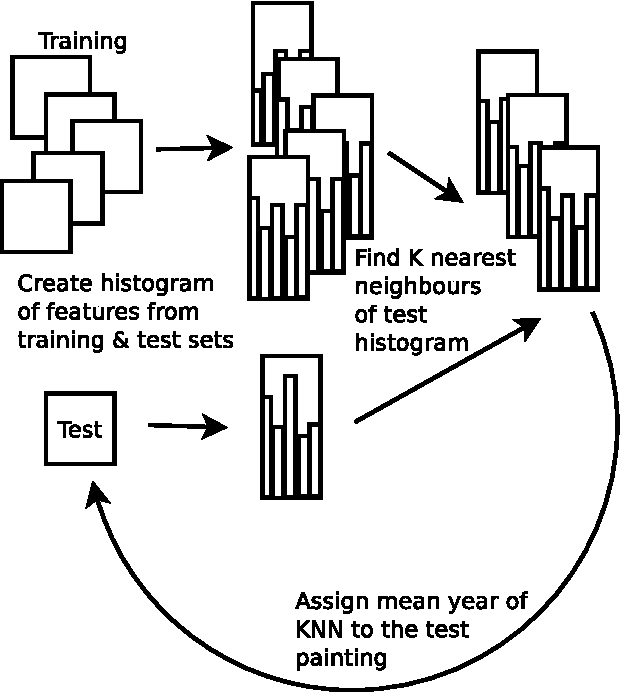
\includegraphics[width=0.4\textwidth]{img/kyffin_overview.pdf}
\caption{Overview of the Classification Methodology}
\label{img:classification-overview}
\end{figure}


\section{Overall Architecture}
The basic architecture for any system like this is to load the data in from a source of some form,
apply an analysis technique to each data point then pass this data into the classification system.

From the classification system you should then be able to get the classified and actual year for
each data point which can then have validation performed on it. This architecture is summed up in
figure~\ref{fig:basic-arch}.

\begin{figure}[h]
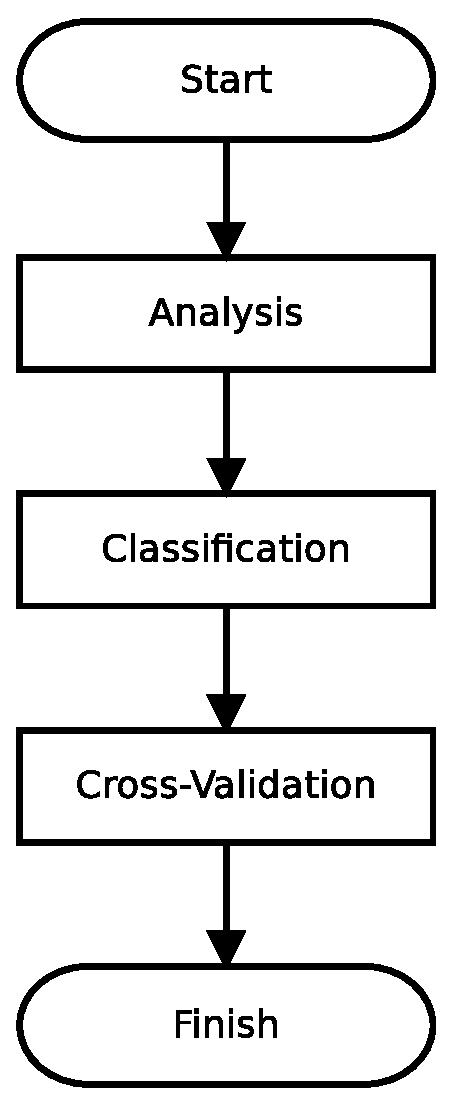
\includegraphics[width=\linewidth]{img/basic-arch}
\caption{Basic Overall Architecture}\label{fig:basic-arch}
\end{figure}

Building up from this it is apparent that to implement the analysis and classification steps that 
there is a need to implement the factory method design 
pattern\cite[p.~107-117]{Gamma1996Design}. Reading from a data source should be a simple
matter of reading from a file, and cross validation has already been decided to use leave-one-out
cross validation.

Figure~\ref{fig:factory-arch} shows the design after adding in the factory methods.

\begin{figure}[h]
\centering
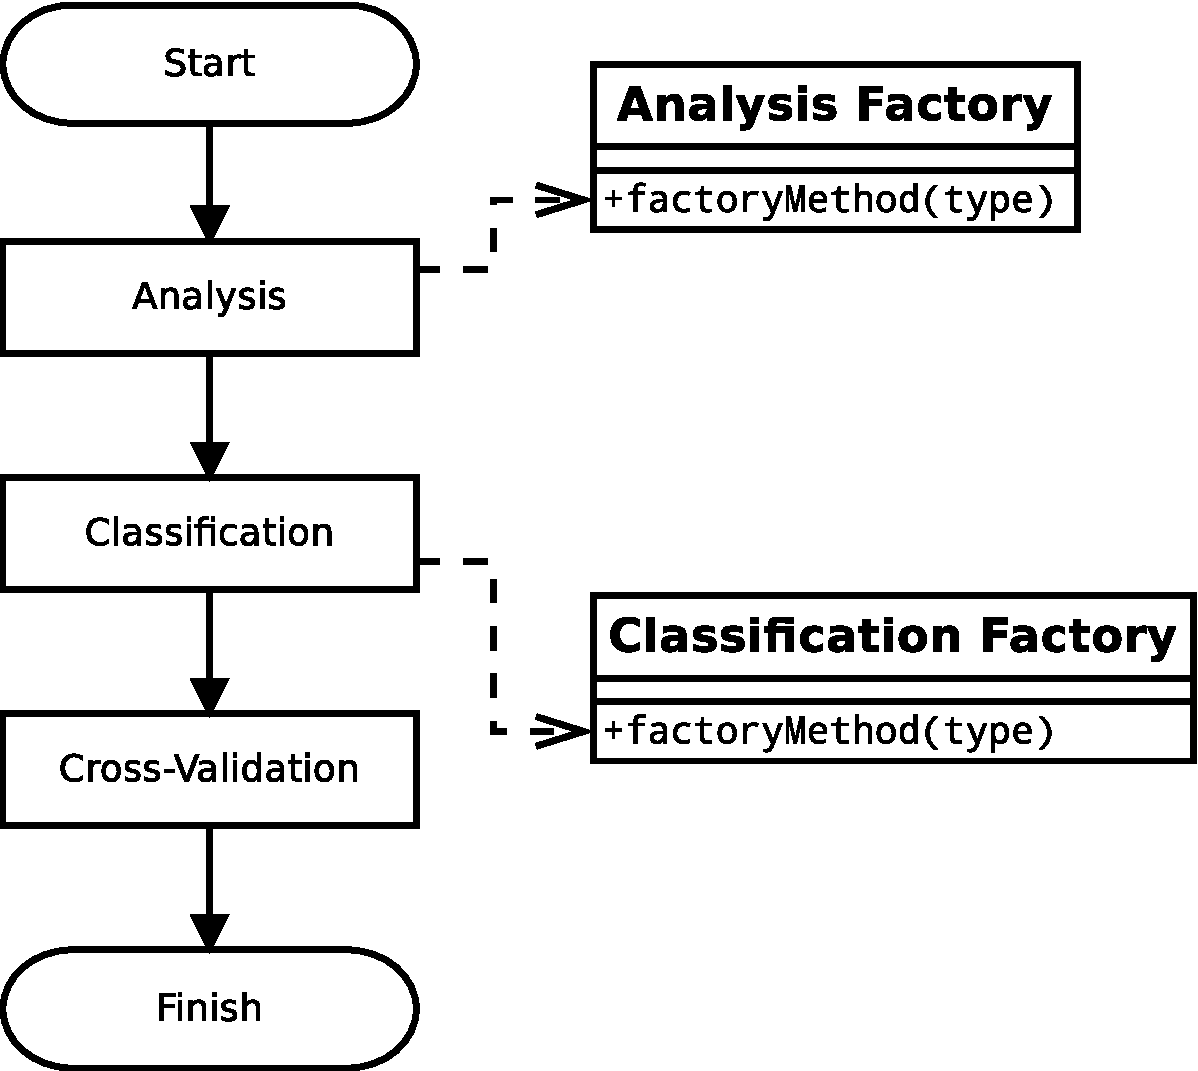
\includegraphics[width=\linewidth]{img/factory-arch}
\caption{Overall Architecture with Factory Methods}\label{fig:factory-arch}
\end{figure}

From this we then need the two top-level interfaces \verb+Analyser+ and \verb+Classifier+. The 
\verb+Analyser+ interface should have a single method which runs analysis on a painting and return
some form of object which represents the analysed data.

The \verb+Classifier+ class should have a method which takes a single painting and a set of
paintings, returning a year which is the classified year of the single painting based on the set
of paintings.

At this point it is also required that there is a class to store meta-data of a painting. 
Figure~\ref{fig:interfaces-arch} depicts the design after adding in these parts.

\begin{figure}[h]
\centering
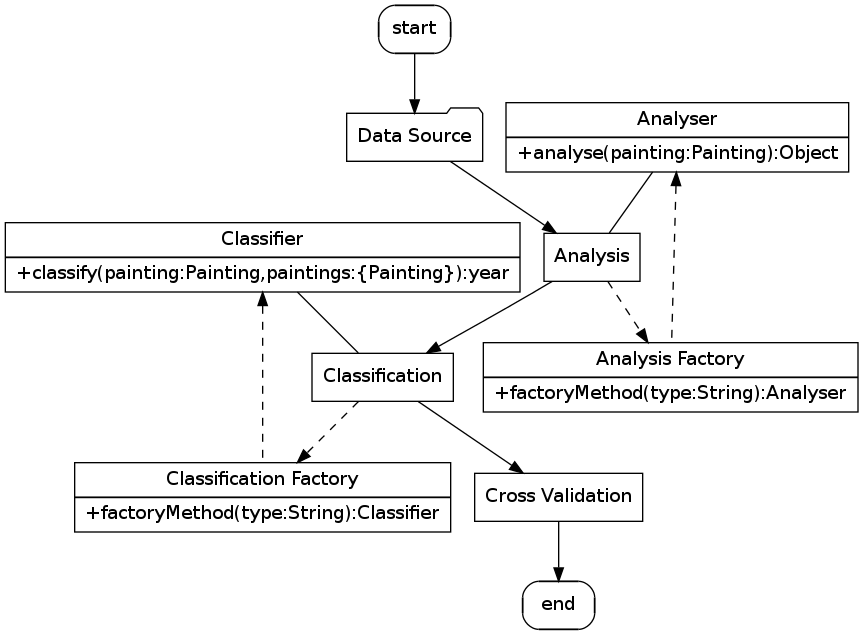
\includegraphics[width=\linewidth]{img/interfaces-arch}
\caption{Overall architecture with Interfaces for Analysers and Classifiers}\label{fig:interfaces-arch}
\end{figure}


